\documentclass[a4paper,12pt]{article} 
\usepackage[utf8]{inputenc} % Acentos válidos sin problemas
\usepackage[spanish]{babel} % Idioma


\usepackage[backend=biber, style=alphabetic, sorting=ynt]{biblatex}
\bibliography{bibliografia.bib}
\nocite{*} % Añade todas las referencias de bib sin cita

%-----------------------------------INICIO DE PACKETES-------------------/
%-----------------------------------------------------------------------/
\usepackage{amsmath}   % Matemáticas: Comandos extras(cajas ecuaciones) |
\usepackage{amsthm}
\usepackage{amssymb}   % Matemáticas: Símbolos matemáticos              |
\usepackage{datetime}  % Agregar fechas                                 |
\usepackage{graphicx}  % Insertar Imágenes                              |
%\usepackage{biblatex} % Bibliografía                                   |
\usepackage{multicol}  % Creación de tablas                             |
\usepackage{longtable} % Tablas más largas                              |
\usepackage{xcolor}    % Permite cambiar colores del texto              |
\usepackage{tcolorbox} % Cajas de color                                 |
\usepackage{setspace}  % Usar espacios                                  |
\usepackage{fancyhdr}  % Para agregar encabezado y pie de página        |
\usepackage{lastpage}  %                                                 |
\usepackage{float}     % Flotantes                                      |
\usepackage{soul}      % "Efectos" en palabras                          |
\usepackage{hyperref}  % Para usar hipervínculos                        |
\usepackage{caption}   % Utilizar las referencias                       |
\usepackage{subcaption} % Poder usar subfiguras                         |
\usepackage{multirow}  % Nos permite modificar tablas                   |
\usepackage{array}     % Permite utilizar los valores para multicolumn  |
\usepackage{booktabs}  % Permite modificar tablas                       |
\usepackage{diagbox}   % Diagonales para las tablas                     |
\usepackage{colortbl}  % Color para tablas                              |
\usepackage{listings}  % Escribir código                               |
\usepackage{mathtools} % SIMBOLO :=                                     |
\usepackage{enumitem}  % Modificar items de Listas                      |
\usepackage{tikz}      %                                                |
\usepackage{lipsum}    % for auto generating text                       |
\usepackage{afterpage} % for "\afterpage"s                              |
\usepackage{pagecolor} % With option pagecolor={somecolor or none}|     |
\usepackage{xpatch}    % Color de lineas C & F
%\usepackage{glossaries} %                                              |
\usepackage{lastpage}    %                                              |   
\usepackage{csquotes}    %                                              |
%-----------------------------------------------------------------------\
%-----------------------------------FIN--- DE PACKETES-------------------\

\usepackage{pgfplots}     %                                             |
\pgfplotsset{compat=1.18} %           
\usepackage{etoolbox}
\usepackage{tikz,times}
\usepackage{verbatim}
\usetikzlibrary{mindmap,trees,backgrounds}
%--------------------------------/
%-------------------------------/
\usepackage[                 %   |
  headheight=15pt,  %            |
  letterpaper,  % Tipo de pag.   |
  left =1.5cm,  %  < 1 >         |
  right =1.5cm, %  < 1 >         | MARGENES DE LA PAGINA
  top =2cm,     %  < 1.5 >       |
  bottom =1.5cm %  < 1.5 >       |
]{geometry}     %                |
%-------------------------------\
%--------------------------------\

%----------------------------------------------------------------------/
%-------------------Encabezado y Pie de Pagina-----------------------/ |
%--------------------------------------------------------------------\ |
%\fancyhf{}
%\pagestyle{fancy}

\fancypagestyle{firstpage}{  
    \fancyhead[L]{}
    \fancyhead[R]{}     
    \fancyfoot[L]{}
    \fancyfoot[C]{}
    \fancyfoot[R]{\thepage\ de \pageref*{LastPage}}    
    \renewcommand{\headrulewidth}{0pt} 
    \xpretocmd\headrule{}{}{\PatchFailed}
}

\fancypagestyle{fancy}{  
    \fancyhead[L]{\textbf{Semestre: 2024-2}}
    \fancyhead[C]{}     
    \fancyhead[R]{}     

    \fancyfoot[L]{\texttt{Skynet Scribes}}
    \fancyfoot[C]{\texttt{IA}}
    \fancyfoot[R]{\thepage\ de \pageref*{LastPage}}

    \renewcommand{\headrulewidth}{1pt} 
    \xpretocmd\headrule{}{}{\PatchFailed}
    \renewcommand{\footrulewidth}{1.5pt} 
    \xpretocmd\footrule{}{}{\PatchFailed}
}

\fancypagestyle{fancyref}{  
    \fancyhead[L]{}
    \fancyhead[R]{}     
    \fancyfoot[L]{\texttt{Skynet Scribes}}
    \fancyfoot[C]{\texttt{IA}}
    \fancyfoot[R]{\thepage\ de \pageref*{LastPage}}    
    \renewcommand{\headrulewidth}{0pt} 
    \xpretocmd\headrule{}{}{\PatchFailed}
}
%--------------------------------------------------------------------\ |
%-------------------Encabezado y Pie de Pagina-----------------------/ |
%------------------------------------------------------------FIN----/


%--------------------------------------------------------------------/
%------------------- LISTA DE COLORES ------------------------------/ 
\definecolor{ProcessBlue}{RGB}{0,176,240}
\definecolor{NavyBlue}{RGB}{0,110,184}
\definecolor{Cyan}{RGB}{0,174,239}
\definecolor{MidnightBlue}{RGB}{0,103,49}
\definecolor{ForestGreen}{RGB}{0,155,85}
\definecolor{Goldenrod}{RGB}{255,223,66}
\definecolor{YellowGreen}{RGB}{152,204,112}
\definecolor{Sepia}{RGB}{103,24,0}
\definecolor{Peach}{RGB}{247,150,90}
\definecolor{CarnationPink}{RGB}{242,130,180}
\definecolor{Fuchsia}{RGB}{140,54,140}
\definecolor{WildStrawberry}{RGB}{238,41,103}
\definecolor{blueRY}{RGB}{13,164,245}

\definecolor{Grass}{RGB}{41,238,53}
\definecolor{Meadow}{RGB}{6,243,67}
\definecolor{jellyfish}{RGB}{109,14,130}
\definecolor{rubber}{RGB}{229,27,232}
\definecolor{bullet}{RGB}{225,31,90}
\definecolor{midnight}{RGB}{31,90,225}
\definecolor{sun}{RGB}{241,152,7}
\definecolor{water}{RGB}{16,229,183}

%------------------- COLORES CÓDIGO ---------------------- |
%------------------- COLORES JAVA ---------------------- |
\definecolor{backcolour}{RGB}{6,6,6} 
%\definecolor{backcolour}{RGB}{181,181,181} 
\definecolor{codeclassjava}{RGB}{246,113,59}
\definecolor{codegreen}{RGB}{17,225,48}
\definecolor{codenumizq}{RGB}{17,17,17}
\definecolor{codestringjava}{RGB}{51,240,234}
\definecolor{codesymboljava}{RGB}{255,5,0} 
\definecolor{yellowpoint}{RGB}{244,235,100} 
%------------------- COLORES JAVA ---------------------- |
%------------------- COLORES PYTHON -------------------- |
\definecolor{backcolourPY}{RGB}{6,6,6} 
%\definecolor{backcolour}{RGB}{181,181,181} 
\definecolor{codegreenPY}{RGB}{17,225,48}
\definecolor{codeclassPY}{RGB}{246,113,59}
\definecolor{codenumizq}{RGB}{17,17,17}
\definecolor{codestringPY}{RGB}{90,128,220}
\definecolor{codesymboljava}{RGB}{255,5,0} 
%------------------- COLORES PYTHON -------------------- |
%------------------- COLORES TERMINAL-------------------- |
\definecolor{backcolourTerminal}{rgb}{0.0, 0.0, 0.0} % Negro
\definecolor{codeclassTerminal}{rgb}{1.0, 1.0, 1.0} % Blanco
\definecolor{codestringTerminal}{rgb}{0.0, 0.6, 0.0} % Verde
\definecolor{codecommentTerminal}{rgb}{0.5, 0.5, 0.5} % Gris
\definecolor{codenumizqTerminal}{rgb}{0.0, 0.0, 1.0} % Azul
\definecolor{codeoptionTerminal}{rgb}{0.4, 0.4, 1.0} % Azul claro para opciones
\definecolor{yellowTerminal}{RGB}{238,200,62}
%------------------- COLORES TERMINAL-------------------- |
%------------------- COLORES CÓDIGO ---------------------- |



%------------------- LISTA DE COLORES -------------------------------\
%---------------------------------------------------------------------\

%-------------- ESTILO de Código PYTHON -----------------------------|
\lstdefinestyle{mystylepython}{
    backgroundcolor=\color{backcolourPY},
    commentstyle=\color{codecommentTerminal},
    keywordstyle=\color{blueRY},
    numberstyle=\tiny\color{codenumizq},
    stringstyle=\color{codestringPY},
    basicstyle=\footnotesize\ttfamily\color{white},
    breakatwhitespace=false,
    breaklines=true,
    captionpos=b,
    keepspaces=true,
    numbers=left,
    numbersep=5pt,
    showspaces=false,
    showstringspaces=false,
    showtabs=false,
    tabsize=2,
    escapechar=\&,
    literate=                
        {;}{{\textcolor{yellowpoint}{;}}}1
        {+}{{\textcolor{yellowpoint}{+}}}1
        {-}{{\textcolor{yellowpoint}{-}}}1
        {\{}{{\textcolor{yellowpoint}{\{}}}1
        {\}}{{\textcolor{yellowpoint}{\}}}}1
        {[}{{\textcolor{yellowpoint}{[}}}1
        {]}{{\textcolor{yellowpoint}{]}}}1
        {=}{{\textcolor{yellowpoint}{=}}}1
        {:}{{\textcolor{yellowpoint}{:}}}1
        {<}{{\textcolor{yellowpoint}{<}}}1
        {>}{{\textcolor{yellowpoint}{>}}}1
}
%-------------- ESTILO de Código PYTHON -----------------------------|
%-------------- ESTILO de Código TERMINAL ---------------------------|
\lstdefinestyle{mystyleTerminal}{
    backgroundcolor=\color{backcolourTerminal},
    commentstyle=\color{codecommentTerminal},
    keywordstyle=\color{codeclassTerminal},
    numberstyle=\tiny\color{backcolourTerminal},
    stringstyle=\color{codestringTerminal},
    basicstyle=\footnotesize\ttfamily\color{codeclassTerminal},
    breakatwhitespace=false,
    breaklines=true,
    captionpos=b,
    keepspaces=true,
    numbers=left,
    numbersep=5pt,
    showspaces=false,
    showstringspaces=false,
    showtabs=false,
    tabsize=4,    
    escapechar=\&,
    literate = 
            {--}{{\textcolor{codecommentTerminal}{--}}}2            
}
% Usar el estilo de código
\lstset{style=mystyleTerminal}
%-------------- ESTILO de Código TERMINAL ---------------------------|
\pagestyle{fancy}

\usepackage{algpseudocode}

\begin{document}%----------------------INICIO DOCUMENTO------------|
%------------------------------------------------------------------|
\begin{titlepage}
\center 
\newcommand{\HRule}{\rule{\linewidth}{0.5mm}} 

%---------------------
%	ESCUDO
%---------------------

\includegraphics[width=4.5cm]{IMA/cienciasWhite.png}

%----------------------------
%	TITULO
%----------------------------
\quad \\[0.2cm]
\textsc{\huge Facultad de Ciencias}\\[.6cm] 
\textsc{\huge Inteligencia Artificial}\\[0.5cm]

%-------------
%	TRABAJO
%-------------
\makeatletter
    \HRule \\ [0.4cm]
        { \huge \bfseries Exploradores de laberinto}\\
    \HRule \\ [0.4cm]
    
\vspace{2mm}

%----------------------------
%	Nombre del Equipo
%----------------------------
\begin{flushleft}
    \Large{Equipo:} \texttt{\Large Skynet Scribes}
\end{flushleft}
%----------------------------
%	Número de practica
%----------------------------
\begin{flushleft}
    \Large{Número de practica:} \texttt{\Large 02}\\[0.8cm]
\end{flushleft}


%-------------------
%	AUTORES
%-------------------
\begin{minipage}{0.8\textwidth}
    \begin{flushright}
        \textbf{\large{Carlos Daniel Cortés Jiménez}}\\    
        420004846        
    \end{flushright}
\end{minipage}

\vspace{5mm}

\begin{minipage}{0.4\textwidth}
        \textbf{\large{Sarah Sophía Olivares García}}\\
        318360638
\end{minipage}
\begin{minipage}{0.4\textwidth}
    \begin{flushright}
        \textbf{\large{Marco Silva Huerta}}\\
        316205326        
    \end{flushright}
\end{minipage}

\vspace{5mm}

\begin{minipage}{0.4\textwidth}
        \textbf{\large{Juan Daniel Barrera Holan}}\\    
        417079372
\end{minipage}
\begin{minipage}{0.4\textwidth}
    \begin{flushright}
        \textbf{\large{Laura Itzel Tinoco Miguel}}\\
        316020189
    \end{flushright}
\end{minipage}

\vspace{10mm}
%-------------------
%	PROFESORES
%-------------------

\begin{minipage}{0.8\textwidth}
    \begin{flushleft} \large
        Profesora: Cecilia Reyes Peña\\
        Ayudante teoría: Karem Ramos Calpulalpan \\
        Ayudante laboratorio: Tania Michelle Rubí Rojas\\                    
    \end{flushleft}
\end{minipage}

\vspace{20mm}

\begin{minipage}{0.4\textwidth}
    %---------------
    %	S E M E S T R E
    %---------------
    \textcolor{white}{Semestre}\\
    \large\textbf{Semestre 2024-2}      
\end{minipage}
\begin{minipage}{0.4\textwidth}
    %---------------
    %	F E C H A
    %---------------
    \begin{flushright}
        {\large Fecha de entrega:\\
         \textbf{28 de Febrero del 2024}}
    \end{flushright}
\end{minipage}

\makeatother

\vfill 
\end{titlepage}

\newpage
\tableofcontents

%% Investigación sobre conceptos iniciales
%\newpage
% ----------------------------------------------------------------------------------------\
% ---------------------------------------------------------------------------------------\
% --------------------------------------------------------------------------------------\
\section{Investigación}
% ----------------------------------------------------------------------------------------\
% ---------------------------------------------------------------------------------------\
% Investiga y escribe un breve resumen sobre los algoritmos 
%  SVM (Support Vector Machine),
%  Decision Tree 
%  Random Forest.
% --------------------------------------------------------------------------------------\

% ----------------------------------------------------------------------------------------\
% ---------------------------------------------------------------------------------------\
\subsection{Algoritmos de aprendizaje supervisados}
% ----------------------------------------------------------------------------------------\
% ---------------------------------------------------------------------------------------\

Los algoritmos de aprendizaje supervisado experimentan un conjunto de datos que contiene 
características, pero cada ejemplo también está asociado con una etiqueta u objetivo. 
Por ejemplo, el conjunto de datos de Iris está anotado con la especie de cada planta de iris. 
Un algoritmo de aprendizaje supervisado puede estudiar el conjunto de datos de Iris y aprender 
a clasificar las plantas de iris en tres especies diferentes según sus mediciones.
\cite{Goodfellow-et-al-2016}\\ 

Es decir aprenden a asociar alguna entrada con alguna salida, dado un conjunto de entrenamiento 
de ejemplos de entradas $x$ y salidas $y$. En muchos casos, los resultados y pueden ser difíciles 
de recopilar automáticamente y deben ser proporcionados por un \textit{supervisor} humano, pero 
el término aún se aplica incluso cuando los objetivos establecidos de capacitación se 
recopilaron automáticamente.\cite{Goodfellow-et-al-2016}\\ 

Brevemente el contraste con los algoritmos de aprendizaje no supervisados experimentan un 
conjunto de datos que contiene muchas características y luego aprenden propiedades útiles de 
la estructura de este conjunto de datos. En el contexto del aprendizaje profundo, generalmente 
queremos aprender la distribución de probabilidad completa que generó un conjunto de datos, ya 
sea explícitamente como en la estimación de densidad o implícitamente para tareas como síntesis 
o eliminación de ruido. Algunos otros algoritmos de aprendizaje no supervisados desempeñan otras 
funciones, como el clustering, que consiste en dividir el conjunto de datos en grupos de 
ejemplos similares.\cite{Goodfellow-et-al-2016}\\


% ----------------------------------------------------------------------------------------\
% ---------------------------------------------------------------------------------------\
\subsection{Support Vector Machine}
% ----------------------------------------------------------------------------------------\
% ---------------------------------------------------------------------------------------\

Uno de los enfoques más influyentes para el aprendizaje supervisado es la máquina de vectores 
de soporte. Este modelo es similar a la regresión logística en el sentido de que está 
impulsado por una función lineal $w^{\intercal} x + b$. A diferencia de la regresión logística, 
la máquina de vectores de soporte no proporciona probabilidades, sino que solo emite una 
identidad de clase. La SVM predice que la clase positiva está presente cuando 
$w^{\intercal} x + b$ es positivo. De manera similar, predice que la clase negativa está 
presente cuando $w^{\intercal} x + b$ es negativo.\cite{Goodfellow-et-al-2016} \\ 

Una máquina de vectores de soporte (SVM) es un modelo de aprendizaje automático potente y 
versátil, capaz de realizar clasificación, regresión e incluso detección de novedades 
lineales o no lineales. Las SVM brillan con conjuntos de datos no lineales de tamaño pequeño 
y mediano (es decir, de cientos a miles de instancias), especialmente para tareas de 
clasificación. Sin embargo, como verá, no se adaptan muy bien a conjuntos de datos 
muy grandes. \cite{géron2022hands}\\ 


La idea fundamental detrás de las máquinas de vectores de soporte (SVM) es encontrar el 
hiperplano que mejor separa dos clases en un espacio de características, maximizando el 
margen entre las instancias de entrenamiento más cercanas a él. En términos simples, busca 
la mejor \textit{avenida} que divide dos grupos de puntos en un espacio multidimensional.\\

Por ejemplo, para la tarea de los correos electrónicos, clasificarlos como spam o no spam, 
tenemos un conjunto de datos con correos etiquetados y cada correo tiene características 
como la frecuencia de ciertas palabras clave, la longitud del mensaje, etc. Utilizando SVM, 
el algoritmo busca un hiperplano en este espacio de características que separe claramente 
los correos de spam de los correos legítimos. El margen entre este hiperplano y las 
instancias más cercanas de cada clase es maximizado, lo que ayuda a mejorar la capacidad de 
generalización del modelo.\\

\begin{center}
    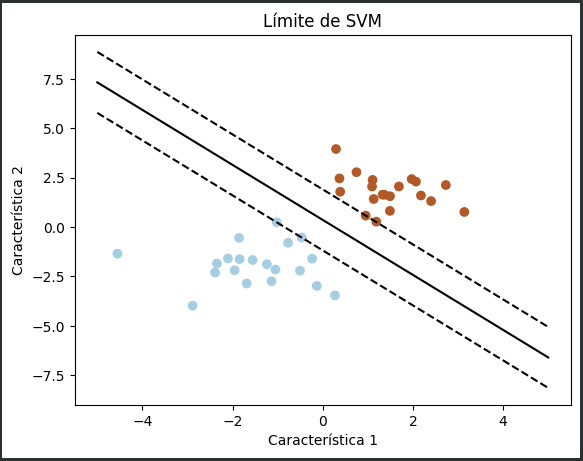
\includegraphics[scale = .5]{IMA/limiteSVM.png}
\end{center}

% ----------------------------------------------------------------------------------------\
% ---------------------------------------------------------------------------------------\
\subsection{Decision Tree}
% ----------------------------------------------------------------------------------------\
% ---------------------------------------------------------------------------------------\

Los árboles de decisión son algoritmos versátiles de aprendizaje automático que pueden 
realizar tareas de clasificación y regresión, e incluso tareas de múltiples salidas. Son 
algoritmos potentes, capaces de ajustar conjuntos de datos complejos. Los árboles de decisión 
también son los componentes fundamentales de los bosques aleatorios, que se encuentran entre 
los algoritmos de aprendizaje automático más poderosos disponibles en la 
actualidad. \cite{géron2022hands}\\ 

El algoritmo puede considerarse no paramétrico si se le permite aprender un árbol de tamaño 
arbitrario, aunque los árboles de decisión generalmente se regularizan con restricciones de 
tamaño que los convierten en modelos paramétricos en la práctica. Los árboles de decisión, 
tal como se utilizan habitualmente, con divisiones alineadas con los ejes y resultados 
constantes dentro de cada nodo, tienen dificultades para resolver algunos problemas que son 
fáciles incluso para la regresión logística. Por ejemplo, si tenemos un problema de dos 
clases y la clase positiva ocurre dondequiera que $x_2 > x_1$, el límite de decisión no 
está alineado con el eje. Por lo tanto, el árbol de decisión necesitará aproximarse al 
límite de decisión con muchos nodos, implementando una función de paso que recorra 
constantemente hacia adelante y hacia atrás a través de la verdadera función de decisión 
con pasos alineados con el eje. \cite{Goodfellow-et-al-2016}

\subsubsection*{Cómo funciona un árbol de decisión.}

\begin{center}
    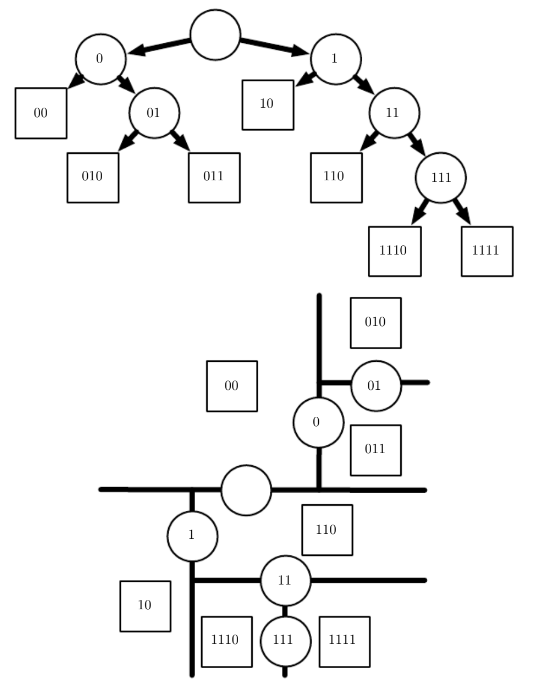
\includegraphics[scale = .7]{IMA/treedesc.png}
\end{center}

Cada nodo del árbol elige enviar el ejemplo de entrada al nodo secundario de la izquierda 
(0) o al nodo secundario de la derecha (1). Los nodos internos se dibujan como círculos y 
los nodos de las hojas como cuadrados. Cada nodo se muestra con un identificador de cadena 
binaria correspondiente a su posición en el árbol, que se obtiene agregando un bit a su 
identificador principal (0=elija izquierda o arriba, 1=elija derecha o abajo). (Abajo) 
El árbol divide el espacio en regiones. \\ 

El plano 2D muestra cómo un árbol de decisión podría 
dividir $\mathbb{R}^{2}$. Los nodos del árbol se trazan en este plano, con cada nodo interno 
dibujado a lo largo de la línea divisoria que utiliza para categorizar ejemplos, y los 
nodos de hoja dibujados en el centro de la región de ejemplos que reciben. El resultado es 
una función constante por partes, con una parte por hoja. Cada hoja requiere al menos un 
ejemplo de entrenamiento para definirse, por lo que no es posible que el árbol de decisión 
aprenda una función que tenga más máximos locales que el número de ejemplos de 
entrenamiento. \cite{Goodfellow-et-al-2016}


% ----------------------------------------------------------------------------------------\
% ---------------------------------------------------------------------------------------\
\subsection{Random Forest}
% ----------------------------------------------------------------------------------------\
% ---------------------------------------------------------------------------------------\

El concepto de sabiduría de la multitud se refiere a la idea de que la respuesta colectiva 
de un grupo de personas al azar a menudo supera la respuesta individual de un experto. 
De manera similar, en el aprendizaje conjunto, al combinar las predicciones de múltiples 
predictores, como clasificadores o regresores, se obtienen predicciones más precisas que 
las de un único predictor. Por lo tanto, el aprendizaje conjunto implica el uso de algoritmos 
que combinan múltiples predictores para mejorar la precisión y la robustez de las predicciones.\\ 

Que significa todo lo de arriba? Los Random Forest (bosques aleatorios) es un algoritmo de 
aprendizaje supervisado que crea un bosque y lo hace de alguna manera aleatorio. Para decirlo 
en palabras simples: el bosque aleatorio crea múltiples árboles de decisión y los combina para 
obtener una predicción más precisa y estable. \cite{Machinelearning}\\

Como ejemplo de método de conjunto, puede entrenar un grupo de clasificadores de árboles de 
decisión, cada uno en un subconjunto aleatorio diferente del conjunto de entrenamiento. 
Luego puede obtener las predicciones de todos los árboles individuales, y la clase que obtiene 
más votos es la predicción del conjunto. Este conjunto de árboles de decisión se denomina 
\textbf{bosque aleatorio} y, a pesar de su simplicidad, es uno de los algoritmos de 
aprendizaje automático más potentes. \cite{géron2022hands}\\ 

Entonces un bosque aleatorio es un conjunto de árboles de decisión, generalmente entrenados 
mediante el método de embolsado, normalmente con $max\_samples$ establecido en el tamaño del 
conjunto de entrenamiento. En lugar de crear un BaggingClassifier y pasarle un 
DecisionTreeClassifier, puede usar la clase \textbf{RandomForestClassifier}, que es más 
conveniente y está optimizada para árboles de decisión (de manera similar, existe una clase 
RandomForestRegressor para tareas de regresión). El siguiente código es un ejemplo de como  
entrena un clasificador de bosque aleatorio con 500 árboles, cada uno limitado a un máximo de 
16 nodos hoja, utilizando todos los núcleos de CPU disponibles:\cite{géron2022hands}\\ 

\begin{lstlisting}[style=mystylepython, language=Python, caption=bosque aleatorio con 500 árboles]
    from sklearn.ensemble import RandomForestClassifier

    rnd_clf = RandomForestClassifier(n_estimators=500, max_leaf_nodes=16, n_jobs=-1, random_state=42)

    rnd_clf.fit(X_train, y_train)

    y_pred_rf = rnd_clf.predict(X_test)    
\end{lstlisting}
%-------------------------------------------

%% Desarrollo sobre el trabajo realizado
%\newpage
% ----------------------------------------------------------------------------------------\
% ---------------------------------------------------------------------------------------\
% --------------------------------------------------------------------------------------\
\section{Desarrollo}
% ----------------------------------------------------------------------------------------\
% ---------------------------------------------------------------------------------------\
% --------------------------------------------------------------------------------------\
% Explicación de las implementaciones, diagrama de flujo, ideas, comentarios, investigación, etc
% ----------------------------------------------------------------------------------------\
% ---------------------------------------------------------------------------------------\
\subsection{Implementación básica del Juego de la Vida}
% ----------------------------------------------------------------------------------------\
% ---------------------------------------------------------------------------------------\



% ----------------------------------------------------------------------------------------\
% ---------------------------------------------------------------------------------------\
\subsection{Introducción a los Algoritmos Genéticos}
% ----------------------------------------------------------------------------------------\
% ---------------------------------------------------------------------------------------\



% ----------------------------------------------------------------------------------------\
% ---------------------------------------------------------------------------------------\
\subsection{Implementación de Algoritmos Genéticos en el Juego de la Vida}
% ----------------------------------------------------------------------------------------\
% ---------------------------------------------------------------------------------------\
%-------------------------------------------

%% Ilustración de las pruebas realizadas
% ----------------------------------------------------------------------------------------\
% ---------------------------------------------------------------------------------------\
% --------------------------------------------------------------------------------------\
\section{Resultados obtenidos}
% ----------------------------------------------------------------------------------------\
% ---------------------------------------------------------------------------------------\
% --------------------------------------------------------------------------------------\
% Mostrar ejecuciones del código con capturas 
% Mostrar una comparación del código

% ----------------------------------------------------------------------------------------\
% ---------------------------------------------------------------------------------------\
\subsection{Implementación básica del Juego de la Vida}
% ----------------------------------------------------------------------------------------\
% ---------------------------------------------------------------------------------------\




% ----------------------------------------------------------------------------------------\
% ---------------------------------------------------------------------------------------\
\subsection{Implementación de Algoritmos Genéticos en el Juego de la Vida}
% ----------------------------------------------------------------------------------------\
% ---------------------------------------------------------------------------------------\




% ----------------------------------------------------------------------------------------\
% ---------------------------------------------------------------------------------------\
% --------------------------------------------------------------------------------------\
\section{Reflexión final}
% ----------------------------------------------------------------------------------------\
% ---------------------------------------------------------------------------------------\
% --------------------------------------------------------------------------------------\

% Después de las simulaciones, analizar cómo la evolución de los cromosomas afectó el 
% desarrollo del Juego de la Vida, identificando patrones o estrategias exitosas.

% Redactar un breve informe que reflexione sobre el aprendizaje obtenido, las estrategias 
% que resultaron ser más efectivas y cómo los principios de los algoritmos genéticos 
% podrían aplicarse a otros problemas de optimización o simulación.
%-------------------------------------------

%% Análisis del equipo 
\subsection{Análisis equipo}

\begin{itemize}
    \item Marco Silva Huerta 
    
    Para el modelo de Logistic Regression su matriz de confusión muestra un rendimiento bastante bueno con un bajo número de 
    falsos positivos y falsos negativos, eso le da un equilibrio del $91\%$ en la clasificación de ham y spam. Pero para el 
    modelo SVM la precisión en números es del $0.9343$, esto pasa porque SVM tiene menos falsos positivos que Logistic Regression.\\ 

    Ahora cuando volteamos a ver a Decision Tree Classifier, muestra un desempeño aceptable en relación a los dos primeros 
    pues cuenta  con un $87\%$ de exactitud general, esto se pude explicar ya que Los árboles de decisión son propensos al 
    sobreajuste cuando se entrenan con conjuntos de datos complejos o desbalanceados ya que sus nodos al dividirse pueden 
    tener dificultades para  generalizar patrones en datos que no han visto durante el entrenamiento.\\ 

    Finalmente el modelo Random Forest Classifier muestra un rendimiento muy muy bueno, fue el que mayor positivos verdaderos tuvo 
    con 1163 y pese a tener también un $93\%$ en la exactitud del modelo, queda segundo lugar pues tiene un $0.9318$, ligeramente 
    por debajo de SVM pero arriba de su individual árbol de decisión, esto porque Random Forest utiliza múltiples árboles de decisión 
    en lugar de uno solo, la combinación de las predicciones reduce el riesgo de sobreajuste.\\ 

    \item Fernando Mendoza Eslava

    El ajuste de \texttt{class\_weight='balanced'} ha sido esencial en nuestros modelos, permitiendo que estos presten más atención a la clase 
    minoritaria 'spam'. Este enfoque ha ayudado a mejorar el \textit{recall} de la clase minoritaria sin sacrificar significativamente la precisión, 
    un balance crucial en aplicaciones reales donde el costo de predecir erróneamente un 'spam' como 'ham' puede ser alto.
    
    Elegimos utilizar \texttt{TfidfVectorizer} por su capacidad para no solo contar la frecuencia de palabras, sino también ajustar estos conteos 
    basándose en la importancia de las palabras dentro del corpus total del documento. Esta técnica ha probado ser efectiva en resaltar 
    las palabras más relevantes y en minimizar el ruido proveniente de palabras comunes pero irrelevantes.
    
    La evaluación detallada utilizando precisión, \textit{recall}, \textit{F1-score} y matrices de confusión ha revelado la robustez de los modelos SVM y 
    Random Forest, que han mostrado un excelente balance entre precisión y capacidad de \textit{recall}. Estas métricas son fundamentales para 
    entender el verdadero rendimiento en un escenario de clases desbalanceadas.

    \item Carlos Daniel Cortés Jiménez

    Notemos que los modelos como \textit{Random Forest Classifier}, \textit{Logistic Regression} y \textit{Support Vector Machine (SVM)} estos 
    presentan un mejor rendimiendo a comparación del modelo \textit{Decision Tree Classifier} aunque la diferencia no sea tan grande, además 
    la tasa de verdaderos positivos con la que se puede detectar mejor mensajes de tipo ham es el modelo \textit{Random Forest Classifier} con 
    una precisión del $95\%$. Por otro lado el modelo con la mejor detección de mensajes de tipo spam es \textit{Support Vector Machine (SVM)} 
    con un porcentaje del $96\%$.

    Podemos decir entonces que los modelos que tienen el mejor equilibrio entre precisión y recall(sensibilidad) son los mdelos anteriores 
    mencionados siendo Random Forest Classifier y \textit{Support Vector Machine (SVM)}, con porcentajes altos de detección de mensajes 
    de tipo spam y ham, siendo lo que deberiamos de usar a la hora de desarrollar programas que tengan el mejor rendimiento y la mejor precisión.

    \item Sarah Sophía Olivares García

    El modelo de Regresión Logística alcanzó una precisión del $91\%$ y un recall del $92\%$ para la clase spam, con una precisión y         recall del $92\%$ y $91\%$ respectivamente para la clase ham. El F1-score general fue del $91\%$.

    El modelo SVM logró una precisión del $93.43\%$ y un recall del $95\%$ para la clase spam, con una precisión y recall del $95\%$ y         $93.43\%$ respectivamente para la clase ham. El F1-score general fue del $93.21\%$.

    Para el Clasificador de Árboles de Decisión, se obtuvo una precisión del $87\%$ y un recall del $86\%$ para la clase spam, y una         precisión y recall del $88\%$ y $87\%$ respectivamente para la clase ham. El F1-score general fue del $87\%$.

    El Clasificador de Bosques Aleatorios obtuvo una precisión del $95\%$ y un recall del $90\%$ para la clase spam, y una precisión y         recall del $96\%$ y $91\%$ respectivamente para la clase ham. El F1-score general fue del $93\%$.

    Basándonos en las métricas de rendimiento, podemos observar que SVM y Random Forest Classifier mostraron el mejor equilibrio entre         precisión y recall, con una alta capacidad de detección de mensajes de spam y ham

\end{itemize}

%-------------------------------------------

% ----------------------|
% Referencias           |
% Forma de Compilar     |
% pdflatex main.tex     |
% biber main            |
% pdflatex main.tex     |
\newpage %              |
\thispagestyle{fancyref}
% \printbibliography %  |
\printbibliography[heading=bibintoc]
% ----------------------|

\end{document}%----------------------F I N DOCUMENTO---------------|
%------------------------------------------------------------------|
